\documentclass[dvipdfmx]{jsarticle}


\usepackage{tcolorbox}
\usepackage{color}
\usepackage{listings, plistings}

%% ノート/latexメモ
%% http://pepper.is.sci.toho-u.ac.jp/pepper/index.php?%A5%CE%A1%BC%A5%C8%2Flatex%A5%E1%A5%E2

% Java
\lstset{% 
  frame=single,
  backgroundcolor={\color[gray]{.9}},
  stringstyle={\ttfamily \color[rgb]{0,0,1}},
  commentstyle={\itshape \color[cmyk]{1,0,1,0}},
  identifierstyle={\ttfamily}, 
  keywordstyle={\ttfamily \color[cmyk]{0,1,0,0}},
  basicstyle={\ttfamily},
  breaklines=true,
  xleftmargin=0zw,
  xrightmargin=0zw,
  framerule=.2pt,
  columns=[l]{fullflexible},
  numbers=left,
  stepnumber=1,
  numberstyle={\scriptsize},
  numbersep=1em,
  language={Java},
  lineskip=-0.5zw,
  morecomment={[s][{\color[cmyk]{1,0,0,0}}]{/**}{*/}},
  keepspaces=true,         % 空白の連続をそのままで
  showstringspaces=false,  % 空白字をOFF
}
%\usepackage[dvipdfmx]{graphicx}
\usepackage{url}
\usepackage[dvipdfmx]{hyperref}
\usepackage{amsmath, amssymb}
\usepackage{itembkbx}
\usepackage{eclbkbox}	% required for `\breakbox' (yatex added)
\usepackage{enumerate}
\usepackage{setspace}
\usepackage{multicol}
\usepackage[default]{cantarell}
\usepackage[T1]{fontenc}
\fboxrule=0.5pt
\parindent=1em
\begin{document}

%\anaumeと入力すると穴埋め解答欄が作れるようにしてる。\anaumesmallで小さめの穴埋めになる。
\newcounter{mycounter} % カウンターを作る
\setcounter{mycounter}{0} % カウンターを初期化
\newcommand{\anaume}[1][]{\refstepcounter{mycounter}{#1}{\boxed{\phantom{aa}\themycounter \phantom{aa}}}} %穴埋め問題の空欄作ってる。
\newcommand{\anaumesmall}[1][]{\refstepcounter{mycounter}{#1}{\boxed{\tiny{\phantom{a}\themycounter \phantom{a}}}}}%小さい版作ってる。色々改造できる。

%% 修正時刻: Sun Oct 31 10:15:15 2021


\section{簡単なWebアプリを作成する}

以下のような、簡単なWebアプリを作成してみた。

\begin{lstlisting}[caption=index.html]
 <!doctype html>
 <html lang="ja">
   <head>
     <meta charset="utf-8"/>
     <title>Click me</title>
     <link rel="stylesheet" href="css/onclick.css"/>
   </head>
   <body>
     <h1>Click me</h1>
     <section>
       <button id="start">クリックしてね</button>
       <div id="area">
         <img id="close" src="./img/close.gif" alt="close"/>
         <p>これはクリックすると、文字列を表示するだけのシンプルなプラグインです。<br/>
         プラグインの勉強のために作成しました。</p>
       </div>
     </section>
     <script src="https://ajax.googleapis.com/ajax/libs/jquery/3.6.0/jquery.min.js"></script>
     <script src="js/onclick.js"></script>
   </body>
 </html>
\end{lstlisting}

\begin{multicols}{2}
\begin{lstlisting}[caption=onclick.js]
'use strict';

$(function () {
  $('#start').on('click', function() {
    $('#area').css('display', 'block');
    $('#start').css('display', 'none');
  });

  $('#close').on('click', function() {
    $('#area').css('display', 'none');
    $('#start').css('display', 'block');
  });
});
\end{lstlisting}


\begin{lstlisting}[caption=onclick.css]
@charset "UTF-8";

#area {
  display: none;
}

#start {
  cursor: pointer;
}

#close {
  cursor: pointer;
}
\end{lstlisting}
\end{multicols}

\vspace{3mm}
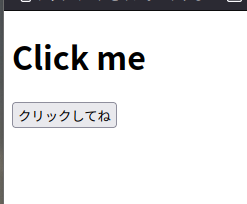
\includegraphics[width=4cm]{img/app01.png}
\vspace{3mm}

\vspace{3mm}
\hspace{10mm}

\includegraphics[width=5mm]{img/arrow-down.png}
\vspace{3mm}


\vspace{3mm}
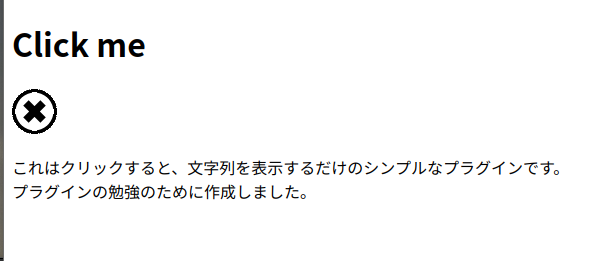
\includegraphics[width=10cm]{img/app02.png}
\vspace{3mm}

フォルダ構成は、以下のとおり。

\begin{spacing}{0.8}
\begin{verbatim}
./onclick-plugin
├── css/
│   └── onclick.css
├── img/
│   └── close.gif
├── index.html
└── js/
    └── onclick.js
\end{verbatim}
\end{spacing}

    


\end{document}

%% 修正時刻: Sat May  2 15:10:04 2020


%% 修正時刻: Sun Oct 31 10:46:56 2021
